\documentclass[a4paper,12pt,pdftex,halfparskip,cleardoubleempty,bibtotoc,liststotoc]{scrbook}

%\raggedbottom

% \usepackage{fancyhdr}

\usepackage[utf8]{inputenc}
\usepackage{wrapfig}
\usepackage[pdftex]{graphicx}
\usepackage{eso-pic}
\usepackage{array}
\usepackage{tabularx}
\usepackage{makecell}
\usepackage{xcolor}
\usepackage{float}
\usepackage{listings}
\usepackage[toc,page]{appendix}
\usepackage[english]{babel}
\usepackage[backend=biber, style=numeric, natbib=true, hyperref=true]{biblatex}

\addbibresource{thesis.bib}

\linespread{1.25}


% chapters, numbering
\newcommand*{\xchapter}{\stepcounter{chapter}\setcounter{section}{0}\addchap}

% tables
\renewcommand\theadalign{bc}
\renewcommand\theadfont{\bfseries}
%\renewcommand\theadgape{\Gape[4pt]}
\renewcommand\cellgape{\Gape[1pt]}
\renewcommand{\arraystretch}{2.5}
\setlength{\tabcolsep}{4pt}

\graphicspath{{img/}}

%\renewcommand*{\thesection}{\arabic{section}}

%\chapterstyle{hangnum}

\definecolor{codegreen}{rgb}{0,0.6,0}
\definecolor{codegray}{rgb}{0.5,0.5,0.5}
\definecolor{codepurple}{rgb}{0.58,0,0.82}
\definecolor{backcolour}{rgb}{0.95,0.95,0.92}

\lstdefinestyle{mystyle}{
    backgroundcolor=\color{backcolour},   
    commentstyle=\color{codegreen},
    keywordstyle=\color{magenta},
    numberstyle=\tiny\color{codegray},
    stringstyle=\color{codepurple},
    basicstyle=\ttfamily\footnotesize,
    breakatwhitespace=false,         
    breaklines=true,                 
    captionpos=b,                    
    keepspaces=true,                 
    numbers=left,                    
    numbersep=5pt,                  
    showspaces=false,                
    showstringspaces=false,
    showtabs=false,                  
    tabsize=2
}

\lstset{style=mystyle}

% define medatata
\def\MTitle{High-Level Modeling and Low-Level Adaptation of Serverless Function Choreographies}
\def\MAuthor{Benjamin Walch}
\def\MKeywords{Serverless \sep Function Choreography Language}
\def\MOrg{Universit{\"a}t Innsbruck}
\def\MDate{\today}
\def\MInstitution{Department of Computer Science}
\def\MSupervisor{Dr. Shashko Ristov}
\def\MGroup{Distributed and Parallel Systems}

%
% \pagestyle{fancy}
% \fancyhf{}
% \fancyhead[L]{\leftmark}
% \fancyhead[R]{\thepage}
% \fancyfoot[R]{B. Walch}
% \fancyfoot[L]{Fastlane}

\pagenumbering{roman}
\begin{document}

\frontmatter
\pagestyle{empty}

\begin{titlepage}
\rule{0mm}{1mm}

\begin{multicols}{2}[\columnsep2em] 
	
\includegraphics[width=6cm]{uibk-logo}
	\columnbreak
	\begin{flushright}
		\Large{\textsf{\MOrg}}
	\end{flushright}
\end{multicols}

\begin{flushright}
	{\large \MInstitution\\}
	{\large \MGroup}
\end{flushright}

\vspace*{1.5cm}

\begin{center}
	{\LARGE\bf \MTitle}
	\vskip 2.25cm
	\Large \textbf{Bachelor Thesis}
	\vskip 2.25cm
	{\Large \MAuthor}
	\vskip 1.5cm
	{\large Supervisor: \MSupervisor}   
	\vfill
	{\large Innsbruck, \MDate}
\end{center}
%\AddToShipoutPicture{
%	\put(-55,55){
%		\parbox[b]{\paperwidth}{
%			\hfill 
\includegraphics[scale=0.35]{uibk-watermark}
%		}
%	}
%}
\end{titlepage} 

\ClearShipoutPicture

\cleardoublepage

\section*{Eidesstaatliche Erklärung}

Ich erkläre hiermit an Eides statt durch meine eigenhändige Unterschrift, dass ich die vorliegende Arbeit selbständig verfasst und keine anderen als die angegebenen Quellen und Hilfsmittel verwendet habe. Alle Stellen, die wörtlich oder inhaltlich den angegebenen Quellen entnommen wurden, sind als solche kenntlich gemacht.

Ich erkläre mich mit der Archivierung der vorliegenden Bachelorarbeit einverstanden.

\vspace{1.8cm}

\parbox{6cm}{
	\hrule
	\strut \centering\footnotesize Datum
} \hfill
\parbox{6cm}{
	\hrule
	\strut \centering\footnotesize Unterschrift
}

\cleardoublepage

\pagestyle{plain}

\chapter*{Abstract}

% to be written at the end!
% some results ..

The Distributed and Parallel Systems group developed the \emph{Abstract Function Choreography Language} (AFCL). It is a specification for describing serverless workflows. Furthermore, a Java API, to describe serverless application workflows programmatically, was developed.
The product which results in using that API is a workflow being described in AFCL in a text based file.
Until now, the workflow being described in the text file has to be created manually (by editing the file directly), or a programmer has to write Java code which utilizes the API to generate the file.
\par
The aim of this bachelor project is to develop a visual workflow editor, which makes modeling of workflows possible at a high level of abstraction. The tool should not only be able to load, display and save workflows, but also optimize workflows for multiple FaaS provider(s) in case of quotas and limits, and also in case of performance.

\cleardoublepage

\tableofcontents

\newpage

\pagenumbering{arabic}

\label{sec:introduction}
\chapter{Introduction}

% - Why is the work important?
% - provider specific implementations
% - need tool to create easily 


% In the FaaS world, there exist many providers who offer serverless execution of code (functions) in the cloud. Each of them has its own specifications and definitions on how functions are deployed and executed, and how workflows are created and executed.
"Run code, not Servers" is a recent term in the cloud computing world.
With the rise of serverless technologies during the last years, \emph{Function-as-a-Service} (FaaS) became more and more popular. This cloud computing concept offers new advantages for software development: very high flexibility, nearly unlimited scalability and pay-per-use pricing. Global Players like Amazon, Google, IBM and Microsoft jumped on the train and provide their infrastructure to developers, with the ability to deploy and execute their code in the cloud. 

Moving from \emph{Infrastucture-as-a-service} (IaaS) over \emph{Platform-as-a-service} (Paas) to Faas, developers can completely focus on the program they need to run and not worry at all about the machine it is on or the resources it requires \cite{articles-going-serverless-savage}.
An entire program can be defined by a workflow, which in turn consists of functions, data dependencies and control structure. Workflows, though, can be executed using serverless technology in the cloud.

But each provider has its own definitions on how a workflow is expressed, as well as different pricing models, limits and quotas. One main issue is the maximum number of concurrent function invocations, which is not more than 1000  for current FaaS providers at time of writing\footnote{checked providers: AWS, Google, IBM and Microsoft}.
Additionally, different providers also support different programming languages. That being said, a workflow from one system is not compatible with another, what means, the user is bound to a specific provider (vendor lock-in), if he wants to reuse or change a workflow later.

\newpage

The distributed and parallel systems group developed a specification to describe serverless workflows at a high abstraction level. This specification is called \emph{Abstract Function Choreography Language} (AFCL) and was created to overcome weaknesses  of current FaaS platforms; for example incompatibility of workflows between different providers.

Although many FaaS providers offer a tool to create a workflow (Amazon Step Functions, IBM Cloud Functions, Microsoft Azure Functions, Google Cloud Functions, ...), building workflows is still a complex task. This is also true for AFCL. Most of the time, this has to be done by a software developer, because others simply lack the neccessary know-how; and even for developers, this task can be tedious and time-consuming.

Castro et al. mentions that "One of the major challenges slowing the adoption of serverless is the lack of tools and frameworks" \cite{articles-rise-of-serverless-castro}. 

Therefore, this thesis has the goal to implement a new tool providing a system, able to model workflows at a high level of abstraction and export them in AFCL. In addition, visualizing - in particular loading, displaying and editing - of existing AFCL workflows in should be supported.
The system should also be able to adapt composed workflows at low-level.

By using the tool, it will be able for non-developers (business guys) to develop a workflow in less time it would take a developer to write the workflow in AFCL.
Another advantage is that exported workflows are compliant with the API and the risk of typos is minimized.
Regarding provider limitations, a scheduler (which is not part of this thesis) should decide to distribute one big concurrent loop - with more iterations than the maximum number of function invocations allowed by the provider - onto multiple FaaS providers. For this purpose, we will provide a service, which offers this low-level adaptation.

% with the GUI it is easier to use the API, such that non-developers can develop an application which is compliant with the API.
% optimization: goal of scheduler is to convert AFCL to CFCL based on the decision which function is executed where. an interface is offered such that the scheduler. Regarding limits of each provider, the scheduler should adapt the workflow to distribute on big loop in multiple providers. For this purpose, we will provide a service, which offers this low-level adaptation.

It is assumed that concrete implementations of the functions are already developed and deployed to a FaaS provider.

%Describing the implementation in the next section 2

%This thesis is structured in three parts. At the beginning there is a short introduction to Faas, followed by explanations and additional information about AFCL.
%After that 

\chapter{Background}

This chapter contains important details on the terms and technologies used in this thesis and helps the reader to better understand the further topics.\\
First of all, the serverless concept, in particular Function-as-a-Service, Serverless Functions and Workflows are explained, before giving a short overview about AFCL. The tools and technologies used for the development are also presented to readers who are not yet familiar with them.

\section{Serverless Computing}

Serverless computing is widely known as an event-driven cloud execution model. In this model, the client provides the code  and the cloud provider manages the life-cycle of the execution environment of that code.
The idea is based on reducing the life span of the program to execute functionality in response to an event. Hence, the program's processes are born when an event is triggered and are killed after the event is processed \cite{inproceedings-serverless-beyond-the-cloud-kanso}.

Castro et al. define serverless computing as follows: "Serverless computing is a platform that hides server usage from developers and runs code on-demand automatically scaled and billed only for the time the code is running" \cite{articles-rise-of-serverless-castro}.

The term ‘serverless’ can be misleading though, as there are still servers providing these backend services, but all of the server space and infrastructure concerns are handled by the vendor. Serverless means that the developers can do their work without having to worry about servers at all \cite{online-what-is-serverless-cloudflare}.

\section{FaaS}

FaaS is a form of serverless computing, which is disrupting the way applications and systems have been built for decades. By abstracting infrastructure provisioning and deployment, user-provided functions can be invoked and executed remotely. The user only has to worry about development and triggering of the function. This serverless runtime has not only the advantage that it avoids costly pre-allocated or dedicated hardware, but also offers almost unlimited possibilities in scalability and billing.

\section{Serverless Functions}
Serverless functions - or tasks - are single-purpose, mostly stateless, programmatic functions that are hosted on cloud infrastructure. These infrastructure is provided through a FaaS platform. They are event-driven and can be invoked through the internet, mainly using HTTP. Like conventional functions, they accept arguments and and return the result of the computation  - with the difference that this is done over a network.

\section{Serverless Workflows}
On an abstract level, a workflow consists of a set of interdependent tasks that need to be executed to achieve a specific goal. [...] A task within a workflow has the following properties: dependencies on the software or service used by the task to perform its computation (software flow), dependencies on data (data flow), and dependencies on other tasks (control flow) \cite{thesis-design-serverless-worfklow-system-eyk}.\\
Basic and advanced control flow patterns for workflows are shown in \cite{reports-workflow-control-patterns-russell}.

A serverless workflow is a complex workflow defined through the composition of serverless functions, connected by control- and data flow. Serverless workflows make it possible to combine and reuse serverless functions in order to build more complex applications. 
Workflows can declare the structure of applications - and using formats like YAML, XML or JSON, they can be described in a text-based file.

\section{AFCL}

Below, a quick overview to AFCL and the control-flow constructs will be given. More detailed information about AFCL will be available soon in a corresponding paper\footnote{At time of writing, \emph{AFCL: An Abstract Function Choreography Language for Serverless Workflow Specification}, by Sasko Ristov et. al was not yet public available}, or in the documentation.\cite{online-afcl-docs-dps}

The \emph{Abstract Function Choreography Language} (AFCL) was created to overcome weaknesses in current FaaS platform implementations. As the name indicates, this specification describes serverless workflows at a high level of abstraction, forming a step on the way to cross-cloud workflow execution.\\
Consider a workflow built with AWS Step Functions, should be executed on IBM Cloud. To make that work, the workflow has to be ported to the other platform to be compatible. In other words - it has to be recreated by a skilled programmer - for example by using the exported workflow as a template.

The AFCL specification has more extensive control-flow and data-flow constructs available than current FaaS providers offer currently in terms of language features. Therefore, AFCL can not only eliminate the incompatibility of workflows between different providers (vendor lock-in), but also opens the door to execute a workflow by distributing its computation over multiple FaaS providers.

To be able to actually execute such multi-cloud workflows, some more tools are needed: an Enactment Engine and a Scheduler.

\subsection{Overview}
% here the different control structures of AFCL?
AFCL is based on YAML\footnote{https://yaml.org} and ships with a schema\footnote{http://dps.uibk.ac.at/projects/afcl/files/schema/schema.yaml}. There exist two types of functions, base functions and compound functions, which can be connected by specifying control-flow and data-flow information. While base functions represent a single task, compound functions provide nesting - they can include some base functions or even other compound functions.

Base and compound functions have data input (dataIns) and data output (dataOuts) ports to define input or output data, respectively.
Data input can refer to data output of another function by specifying the namein combination with the data ouput port of the other function.

\subsection{Control-flow}
In AFCL, base or compound functions are specified one after another, which defines they are executed sequential. However, the following control constructs are introduced with AFCL: \texttt{sequence}, \texttt{if-then-else}, \texttt{switch}, \texttt{for}, \texttt{while}, \texttt{parallel} and \texttt{parallelFor}.


\subsection{Properties and Constraints}

Additional, optional attributes for \{texttt{dataIns} and \texttt{dataOuts} ports of a function, or for the function itself can be defined in \texttt{properties} and \texttt{constraints}. While those are simple key-value pairs accepting string values, AFCL has a few defined properties and constraints to specify concrete attributes like invocation type, element index or data distribution information.

% data flow (dag based)
\subsection{Data-flow}


\section{Development Tools and Technologies}
\subsection{npm}

The node package manager\footnote{https://www.npmjs.org} is the world's largest software registry, where open-source software packages of developers and companies are shared all over the world. Over the last years, npm became a de-facto standard for package management in JavaScript development.

\subsection{webpack}

webpack is a module bundler, its main purpose is to bundle JavaScript code for the usage in a browser.\footnote{https://webpack.js.org} In particular, multiple modules (often hundreds of) with dependencies [to each other] are processed and bundled into a few files. To be able to process other types of files than JavaScript or JSON, webpack offers the opportunity to configure a \textbf{loader}. In this application, the following loaders are configured:
\begin{itemize}
\item babel-loader, to transform ECMAScript and React JSX to browser-compatible JavaScript
\item sass-loader, to transform SASS to CSS
\item css-loader, to transform CSS to CommonJS
\item file-loader, to handle static resources like images and fonts
\end{itemize}

\subsection{ECMAScript}

The scripting language specification ECMAScript (ES) was created to standardize JavaScript. With the release of ES6 (also known as ECMAScript 2015), features like class declarations, module imports and arrow function expressions became possible. After ES6, every year a new edition of the ECMAScript standard was finalized and released, offering new features. Worth mentioning here is the rest/spread operator released with ES9, which occurs a lot in the source code of this thesis.\\
% spread operator is a lot in use in source code
Since current browsers only have partial support of ECMAScript, a 'transcompiler' (or transpiler) is needed to transform the ECMAScript source code to JavaScript, which common browsers are capable of interpreting.
This compiling process is done with Babel\footnote{https://babeljs.io}, which is configured to not only compile ECMAScript, but also JSX to JavaScript.

\subsection{SASS}

CSS, in its pure form, reaches its limits when one thinks about using variables, functions or nested rules. SASS\footnote{https://sass-lang.com} is a stylesheet language, which is - similiar to ES - compiled to CSS and offers the mentioned and even more features.
A lot of CSS Frameworks also provide their source code in SASS, often served with a large variable set which makes it easy to customize it. The transpiler used in this thesis to transform SASS to CSS is node-sass\footnote{https://github.com/sass/node-sass}.


\chapter{Implementation}

% what the system does, what if offers

The main goals for this thesis were the implementation of a tool, which should not only visualize AFCL Workflows, but also give non-developers the opportunity to create and edit workflows through a GUI. This GUI ships with a powerful editor with additional features like real-time validation, versioning and automatic layouting.\\
Furthermore, workflows can be adapted at low-level by dividing concurrency in loops.

The following sections explain the high-level overview architecture and give specific information about how the implementation was done. 

\section{System Architecture}
% what was built

The whole system consists of two sub systems which are operating mostly decoupled from each other: a Java backend and a web-based frontend. Those communicate and share JSON or XML encoded objects between each other through an API the backend provides and the frontend consumes.

The backend is responsible for converting and adapting workflows at low-level as well as persisting of function data.

The frontend displays and controls the application's user interface. It is responsible for visualizing the data and provides the editor with the canvas where a user can compose a workflow.

\subsection{High level overview}

% present only functionalities
% create workflow
% load workflow
% validator
% "versioning" (command history for undo/redo)
% automatic layout from empty YAML/JSON

% Frontend - explain 
% accepts YAML/JSON - visualize it - save or export it

\subsection{Frontend}
% details about frontend

% Architecture "high level overview"
\begin{figure}[htbp]
  \centering
  \vspace{0.8cm}
  \includegraphics[width=0.8\textwidth]{frontend-setup}
  \caption{frontend build stack}
\end{figure}

\subsection{Backend}

The conversion of workflows is needed because the frontend encodes the visual representation of a workflow in XML, which is given as input to the backend. The conversion process is done by utilizing the AFCL API\footnote{http://dps.uibk.ac.at/projects/afcl/files/jar/afclAPI.jar}. 

% interface for adaptation during runtime such that based on the decision of the scheduler also automatic display of new "optimized" workflow

% all this should be visible on the architecture

% show interfaces between modules
% Input output in each
% communication
% (to subsystems: FE constists of this ..., BE constists of this - goals of both BE and FE)
% more grained visualization

% which functional components does the system have!

% put scheduler on the left side in this graphic
% scheduler has interface
\begin{figure}[H]
  \centering
  \vspace{0.8cm}
  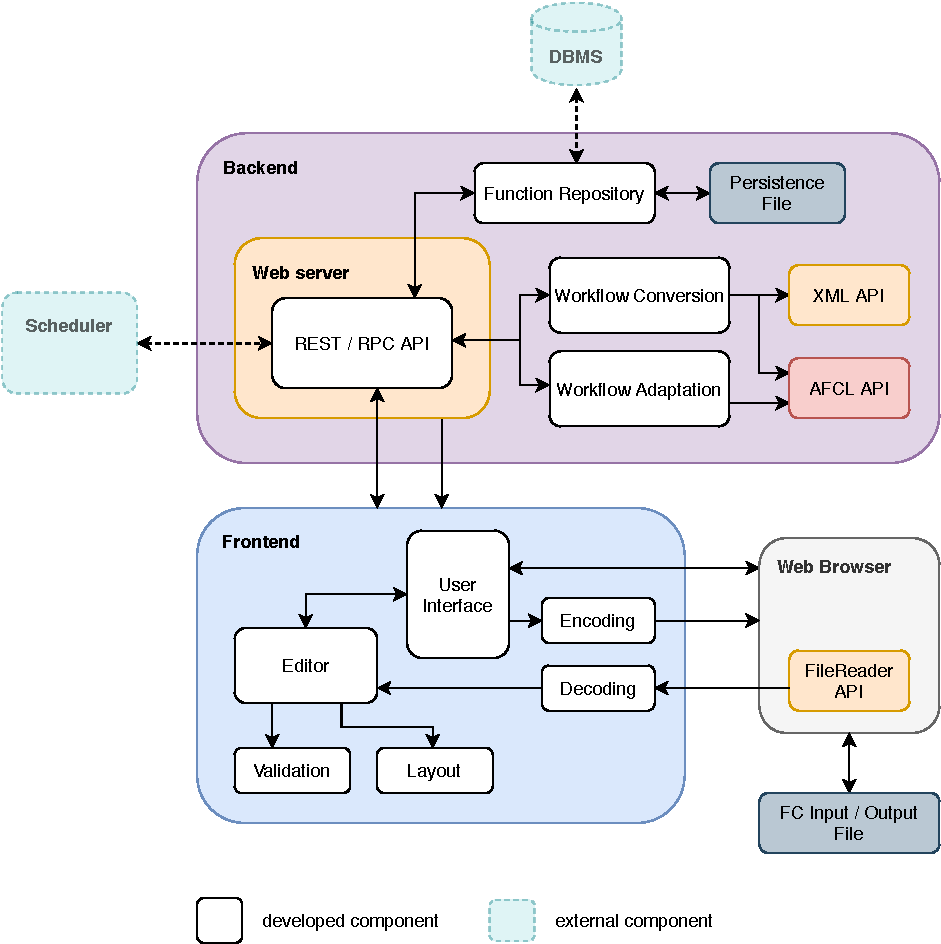
\includegraphics[scale=0.8]{architecture}
  \caption{application architecture}
\end{figure}

\section{System Design}
%how you build / implement it
Since a web based frontend which runs in the user's web browser, is a hard requirement, the core technologies are limited to HTML, CSS and JavaScript.


% \subsection{Development Workflow}
% SYSTEM DESIGN
\subsection{Frontend}

The setup of the frontend application is a selection of tools and technologies for modern and complex web development.
The base forms npm, which is used to manage and resolve dependencies. Additionally, npm's CLI is used as tool to execute development and build tasks. Webpack is in use to bundle all sources and assets into single files, and execute additional build steps by utilizing so-called 'loaders'.

Under the hood, JavaScript and several JavaScript Frameworks are in action to control the application consisting of several UI components. To give the application its look and feel, CSS and some CSS Frameworks are in use.

Babel is used as such a webpack loader, for compiling the ECMAScript and React JSX source code to browser-compatible JavaScript.
The same applies for the CSS extension SASS, which is also integrated as a webpack loader, and is used to make the process of styling the user interface more efficient.

%%% TECHNOLOGIES / TOOLS %%%

\subsubsection{Data model}

All AFCL Java model classes\cite{online-afcl-docs-dps} have been ported to ECMAScript, to have all classes and properties available in the frontend, similiar like they are in the backend. Although plain JavaScript objects would also do the job, this adds a kind of type-safety to the ECMAScript sources and improves readability of the code. Also, the data exchange with the backend and the encoding of the graph benefit from this approach, since the XML node names map to constructor names.

\subsubsection{Graph drawing}

An AFCL workflow can be visualized as a directed acyclic graph (DAG). For reasons of efficiency, reusability, documentation and future safety, there is no question that an existing library has to be used to do the visualizing part.
At the time of implementation, the JavaScript library mxGraph\footnote{https://jgraph.github.io/mxgraph/} was the best choice\footnote{see \ref{sec:graph-alternatives} to learn why} to achieve the mentioned goals.
It has an outstanding documentation, enriched with a lot of demos and example code which show many use cases and extensive features, as well as a powerful production-grade example\footnote{https://draw.io}.\\
The authors of mxGraph state:\\
\begin{quote}
``mxGraph is pretty much feature complete, production tested in many large enterprises and stable for many years. We actively fix bugs and add features [...].''
\end{quote}

In mxGraph, vertices and edges are represented by an \texttt{mxCell} model, which stores information about the cell's position, dimension, geometry and style.

\begin{figure}[H]
  \centering
  \vspace{0.8cm}
  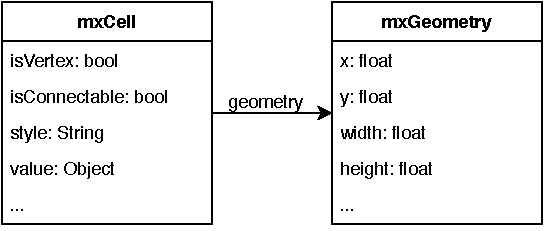
\includegraphics[]{mxCell}
  \caption{\texttt{mxCell} model}
\end{figure}

% \texttt{mxCell} instances are controlled by the \texttt{mxGraphModel}, its visual representation is rendered by \texttt{mxCellRenderer}.
Additionally, a \textit{user object} can be associated with a \texttt{mxCell} through the \texttt{value} property. User objects give the graph its context, they store the business logic associated with the visual part. \cite{manuals-mxgraph-user-manual} For simple cases, the user object may be a string to display the cell's label. In more complex applications, the user object may be an object and some property of that object will generally be the label that the visual cell displays. In this application, the cell's user objects are instances of the ported AFCL classes, respectively.

The following table shows the implemented \texttt{mxCell}'s shapes which are used for composing a workflow. Beside a short description, the type of the associated user object is denoted.

\begin{table}[h]
   \centering
\begin{tabular}{ |c|c|c| } 
\hline
\thead{Cell} & \thead{Description} & \thead{User Object} \\
\hline
\makecell{
\includegraphics[width=32pt,height=32pt]{cell-start} \\ \textsf{Start}}  & Defines the workflow's entry point & \makecell{\texttt{String} \\ \small(for the label)} \\
\hline
\makecell{
\includegraphics[width=32pt,height=32pt]{cell-end} \\ \textsf{End}}  & Defines the workflow's termination & \makecell{\texttt{String} \\ \small(for the label)} \\
\hline
\makecell{
\includegraphics[width=52pt,height=28pt]{cell-function} \\ \textsf{Function}}  & An atomic function & \texttt{AtomicFunction} * \\
\hline
\makecell{
\includegraphics[width=32pt,height=32pt]{cell-ifthenelse} \\ \textsf{If-Then-Else}}  & A mutual exclusive condition & \texttt{IfThenElse} * \\
\hline
\makecell{
\includegraphics[width=32pt,height=32pt]{cell-switch} \\ \textsf{Switch}}  & A multi condition & \texttt{Switch} * \\
\hline
\makecell{
\includegraphics[width=32pt,height=24pt]{cell-merge} \\ \textsf{Merge}}  & An element for merging previous branches & \makecell{\texttt{null} \\ \small(None)} \\
\hline
\makecell{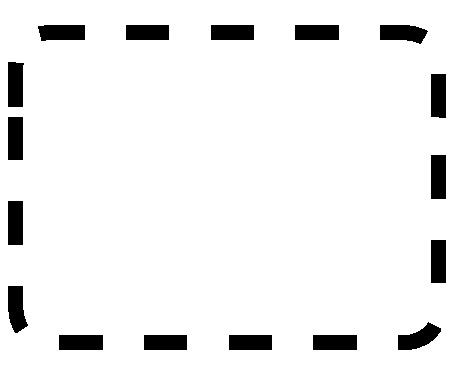
\includegraphics[width=50pt,height=32pt]{cell-compound} \\ \textsf{Parallel}}  & \makecell{A container, where each child cell\\ is meant to be executed in parallel.} & \texttt{Parallel} * \\
\hline
\makecell{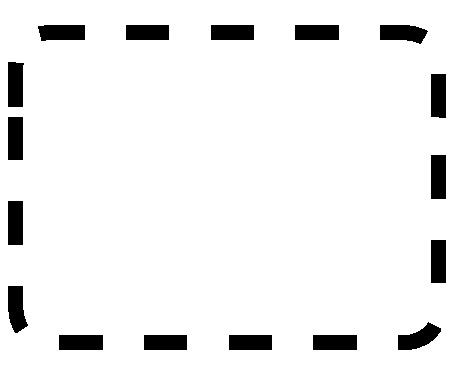
\includegraphics[width=50pt,height=32pt]{cell-compound} \\ \textsf{ParallelFor}}  & \makecell{A container, where each child cell\\ is meant to be executed in a parallel for loop.} & \texttt{ParallelFor} * \\
\hline
\end{tabular}
\caption{Implemented Shapes, *: AFCL Object}
\end{table}

\subsubsection{Validation}

A DAG which represents a valid AFCL workfow always fulfills the following constraints:

\begin{itemize}
	\item There exists exactly one starting point
	\item There exists exactly one termination point
	\item There exist no cycles
	\item Function, If-Then-Else, Switch, Parallel, ParallelFor and End have exactly one incoming edge
	\item Start, Function, Parallel, ParallelFor and Merge have exactly one outgoing edge
	\item IfThenElse has exactly two outgoing edges (then, else)
	\item Switch and Merge have multiple outgoing edges
\end{itemize}

These constraints are enforced at two different stages: At modeling-time, when composing a workflow, more specificially when adding and connecting vertices, and before exporting or adaptation of a workflow.
Due the fact that the user cannot even create an invalid workflow, efficiency increases and errors in the corresponding backend services will be minimized.


\subsection{Encoding}

The visual representation of the workflow and the included data targets human-readability. This data needs to be put into another, proper format for storing. mxGraph provides built-in support for converting the visual representation to XML. An advantage of using XML over JSON is that constructor names (class names) are mapped to the XML node names, no additional property is required.
XML is also very convenient for the backend side, since Java has excellent built-in XML support. The XML-encoded workflow is converted on backend-side internally to an AFCL object.

\subsection{Layouting}

Combination of nested hierarchical layout

\label{sec:graph-alternatives}
\subsection{Alternatives}

One of the more difficult tasks was to choose a proper library for graph drawing. Since the graph drawing and visualization is one of the most important features of the frontend, a careful choice has to be made. Of course there exist multiple excellent JavaScript graph drawing libraries.

Below is a list of tested and researched JavaScript graph libraries with additional information why they were insufficient for the project.
\begin{itemize}
	\item \textbf{jsPlumb} is a library of great quality and looks like it would fulfill all  requirements for graph drawing and user interaction out of the box. It has a very good documentation, and a lot of examples. Furthermore its animations and drag and drop handling are outstandingly good. Unfortunately this software is not open source and a license costs a few thousand dollars.
	\item The same goes for \textbf{Rappid} (formerly known as JointJS) and \textbf{GoJS}, which is even more expensive.
	\item \textbf{diagram-js} is one of the newer diagram libraries. It seems to be a good candidate to draw BPMN\footnote{http://www.bpmn.org} graphs. The lack of an appropriate documentation - even after 4 years of existence (there exists an open issue on github\footnote{https://github.com/bpmn-io/diagram-js/issues/78} for this) - is still an issue.
	\item \textbf{Cytoscape.js} is older than mxGraph but the development and the community is not less active. This library has a very good documentation and a lot of demos are provided. But it offers fewer examples and "out-of-the-box" features for modeling flowcharts than mxGraph does.
	\item \textbf{vis.js} is a star on npmtrends.\footnote{https://www.npmtrends.com/vis}  It has very smooth animations when manipulating the graph. There exists only one example of graph manipulation on its documentation, it is mainly used for visualization only.
	\item \textbf{Sigma js} is a tiny library with a small documentation. It clearly focuses on displaying and visualizing graphs, not on modeling them. This part would have to be developed manually. Furthermore, the last activity on this project on github was 2 years ago.
\end{itemize}

\subsection{Web Interface}

The layout of the web interface is based on coreUI\footnote{https://coreui.io}, an admin panel template, built on top of the web toolkit Bootstrap\footnote{https://getbootstrap.com}. A clean and nested structure of components, which is typical for a React app, guarantees modularity and forms the whole frontend application. One of the benefits when using React is that the data model displayed to the user maps most of the time nicely to UI components. Basically, the components of the application respect the single responsibility principle\footnote{https://en.wikipedia.org/wiki/Single\_responsibility\_principle}. The main component has four sub-components - where each of them consists again of multiple sub-components - representing the core features of the app.

\subsubsection{Dashboard}

The dashboard is the entry point where the user lands after accessing the app. The purpose of this component is to give the user a quick overview of the application, provide short informational texts and links to the specific modules. 

\begin{figure}[H]
  \centering
  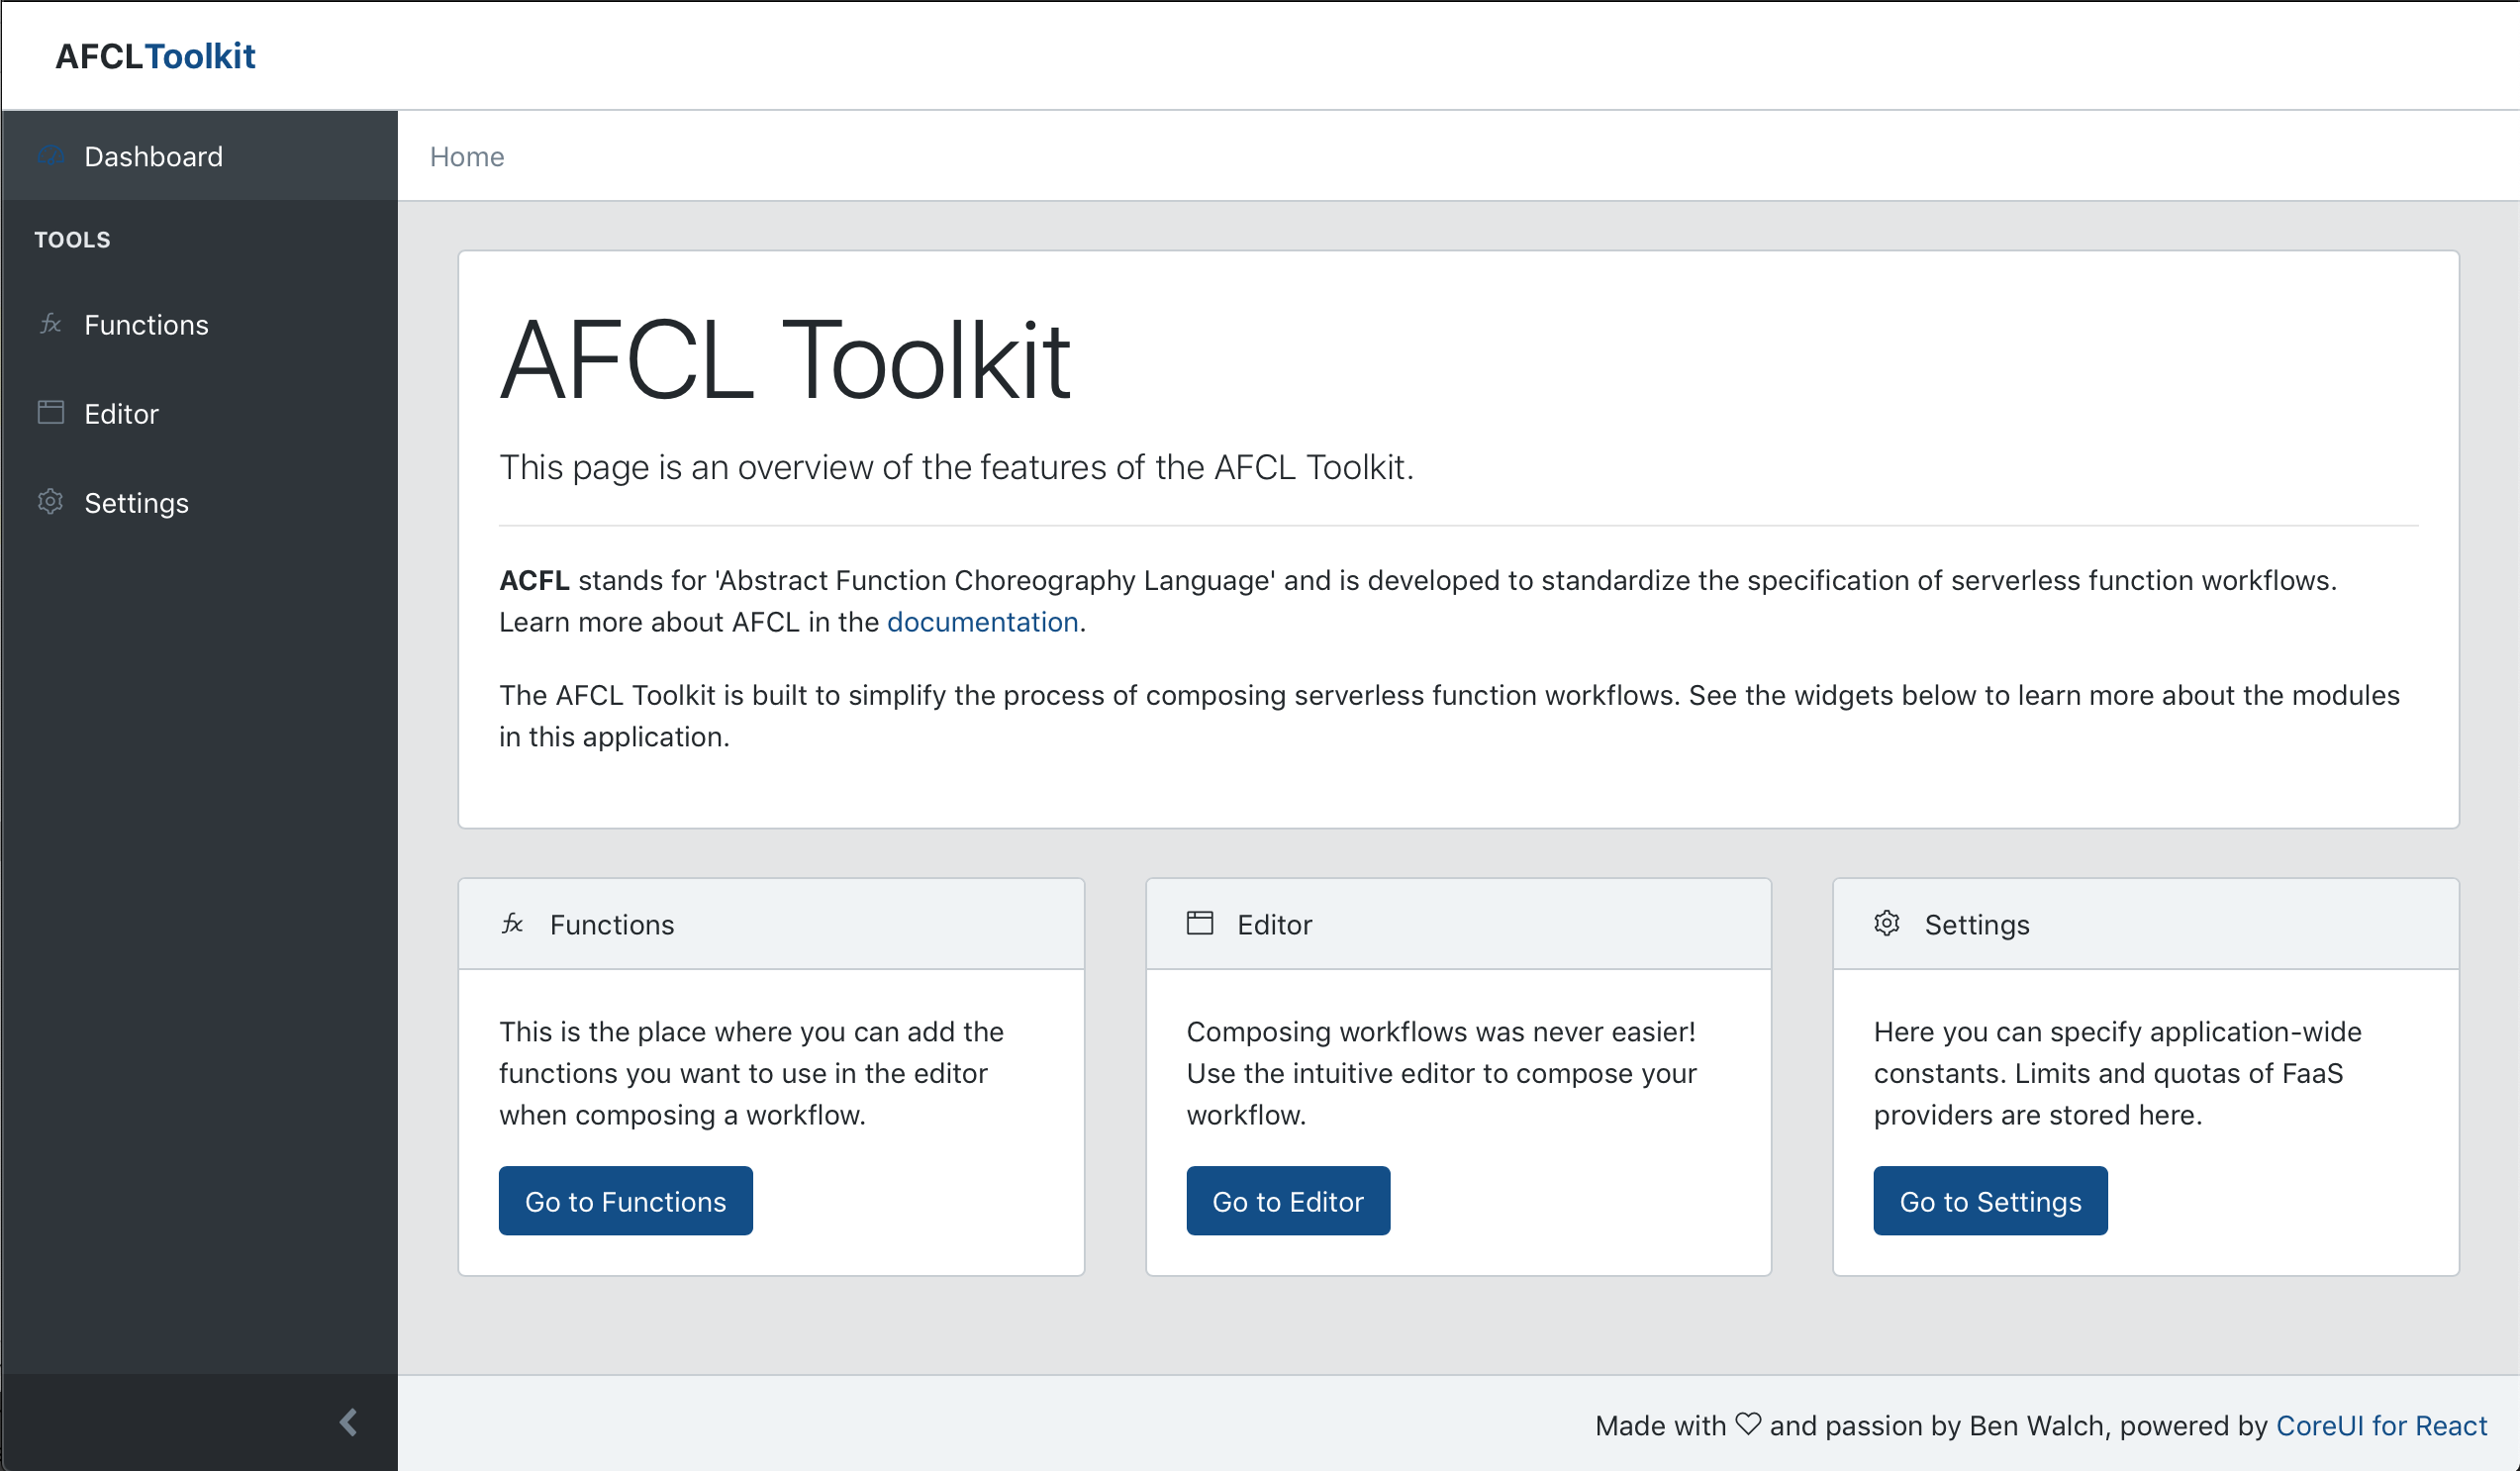
\includegraphics[width=\textwidth]{dashboard}
  \caption{the dashboard}
\end{figure}

\subsubsection{Functions}

A function repository is needed to know about available functions when composing a workflow. An item in the function repository holds the following data: \texttt{name}, \texttt{type} and \texttt{provider}. In the implementation of this thesis, this data is persisted to an internal file.\footnote{see \ref{sec:backend-persistence} for detailed information on how data is persisted}

\begin{figure}[H]
  \centering
  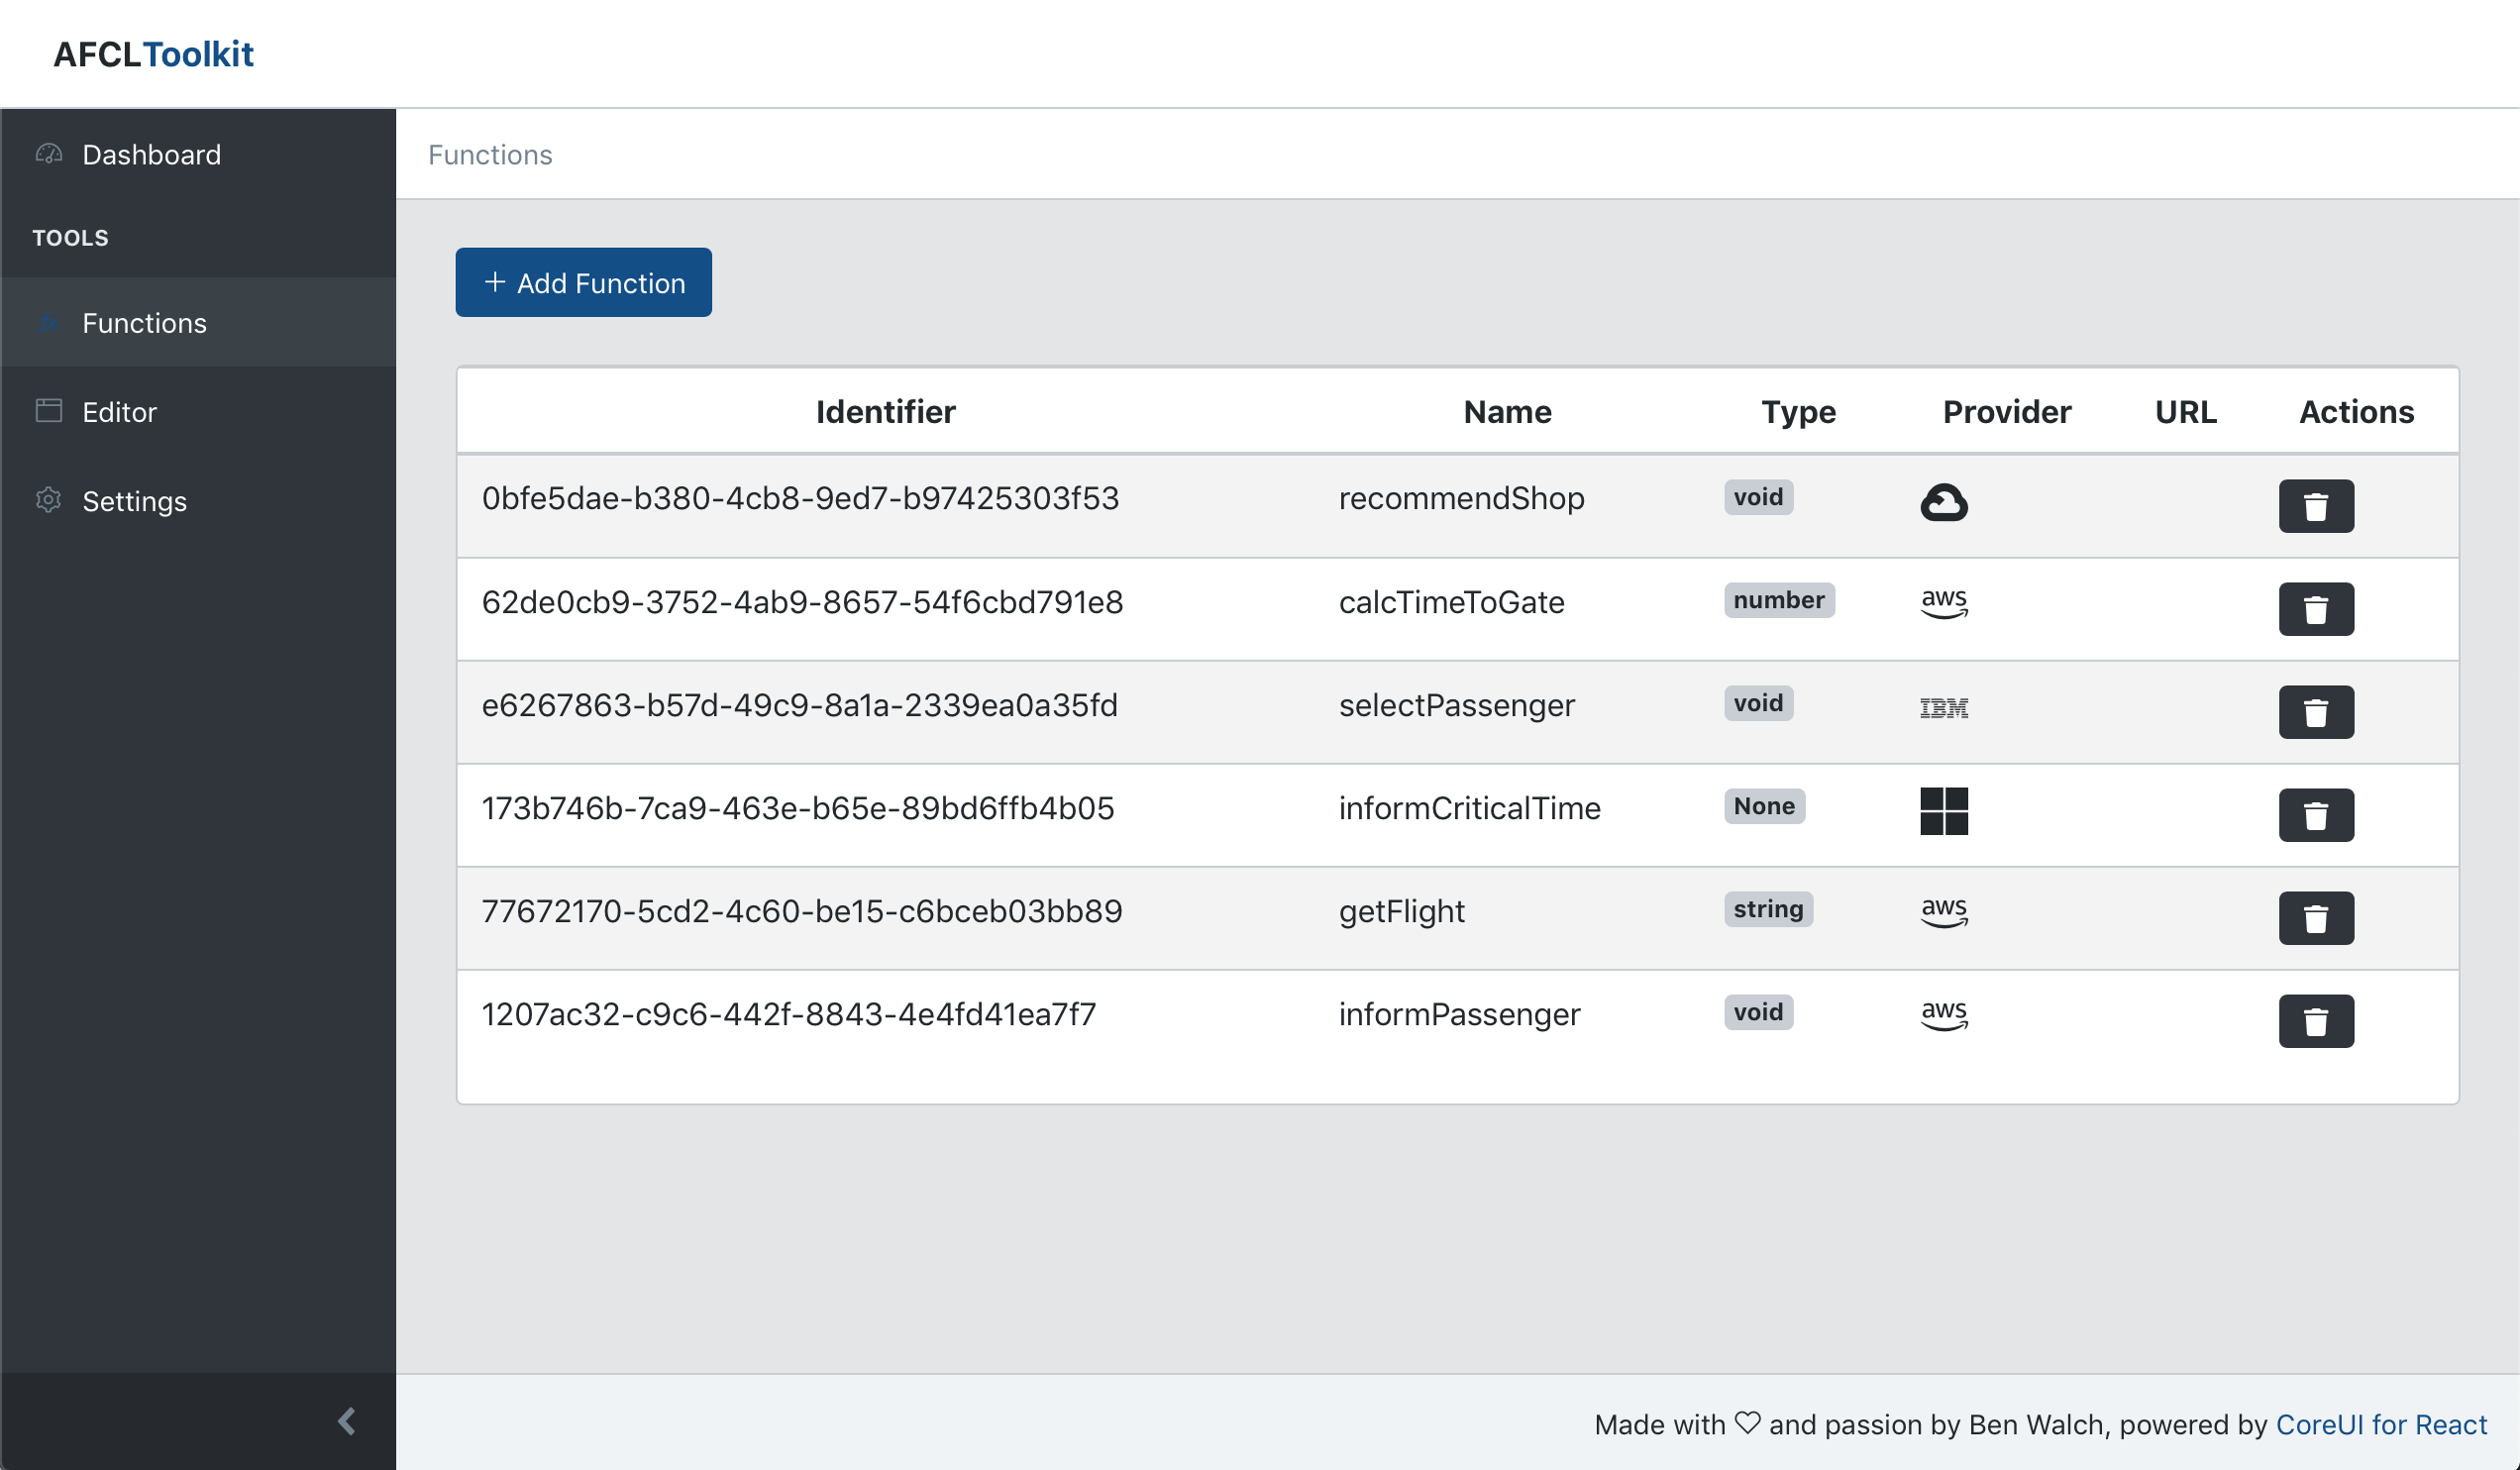
\includegraphics[width=\textwidth]{functions}
  \caption{the function repository}
\end{figure}

\subsubsection{Editor}
\par
The interface of the component responsible for composing workflows is divided into two parts. On the left side is the editor, consisting of a toolbar and a drawing area, on the right side is the property view. In the editor, the user can choose a function from the toolbar to place it in the drawing area below.  For the sake of clarity, each function has a defined shape and style. In the drawing area, these shapes (functions) can then be connected to each other by drag and drop. This leads to a directed graph, which represent the execution flow. The possible connection points (ports) of a shape will be displayed when hovering over it. These ports are input and output for most of the functions. When hovering a port, the port name appears in the tooltip.
\par
When selecting a shape in the canvas, the property view changes. It displays each specific property of the selected function, with the ability to change, add or remove properties.

\begin{figure}[H]
  \centering
  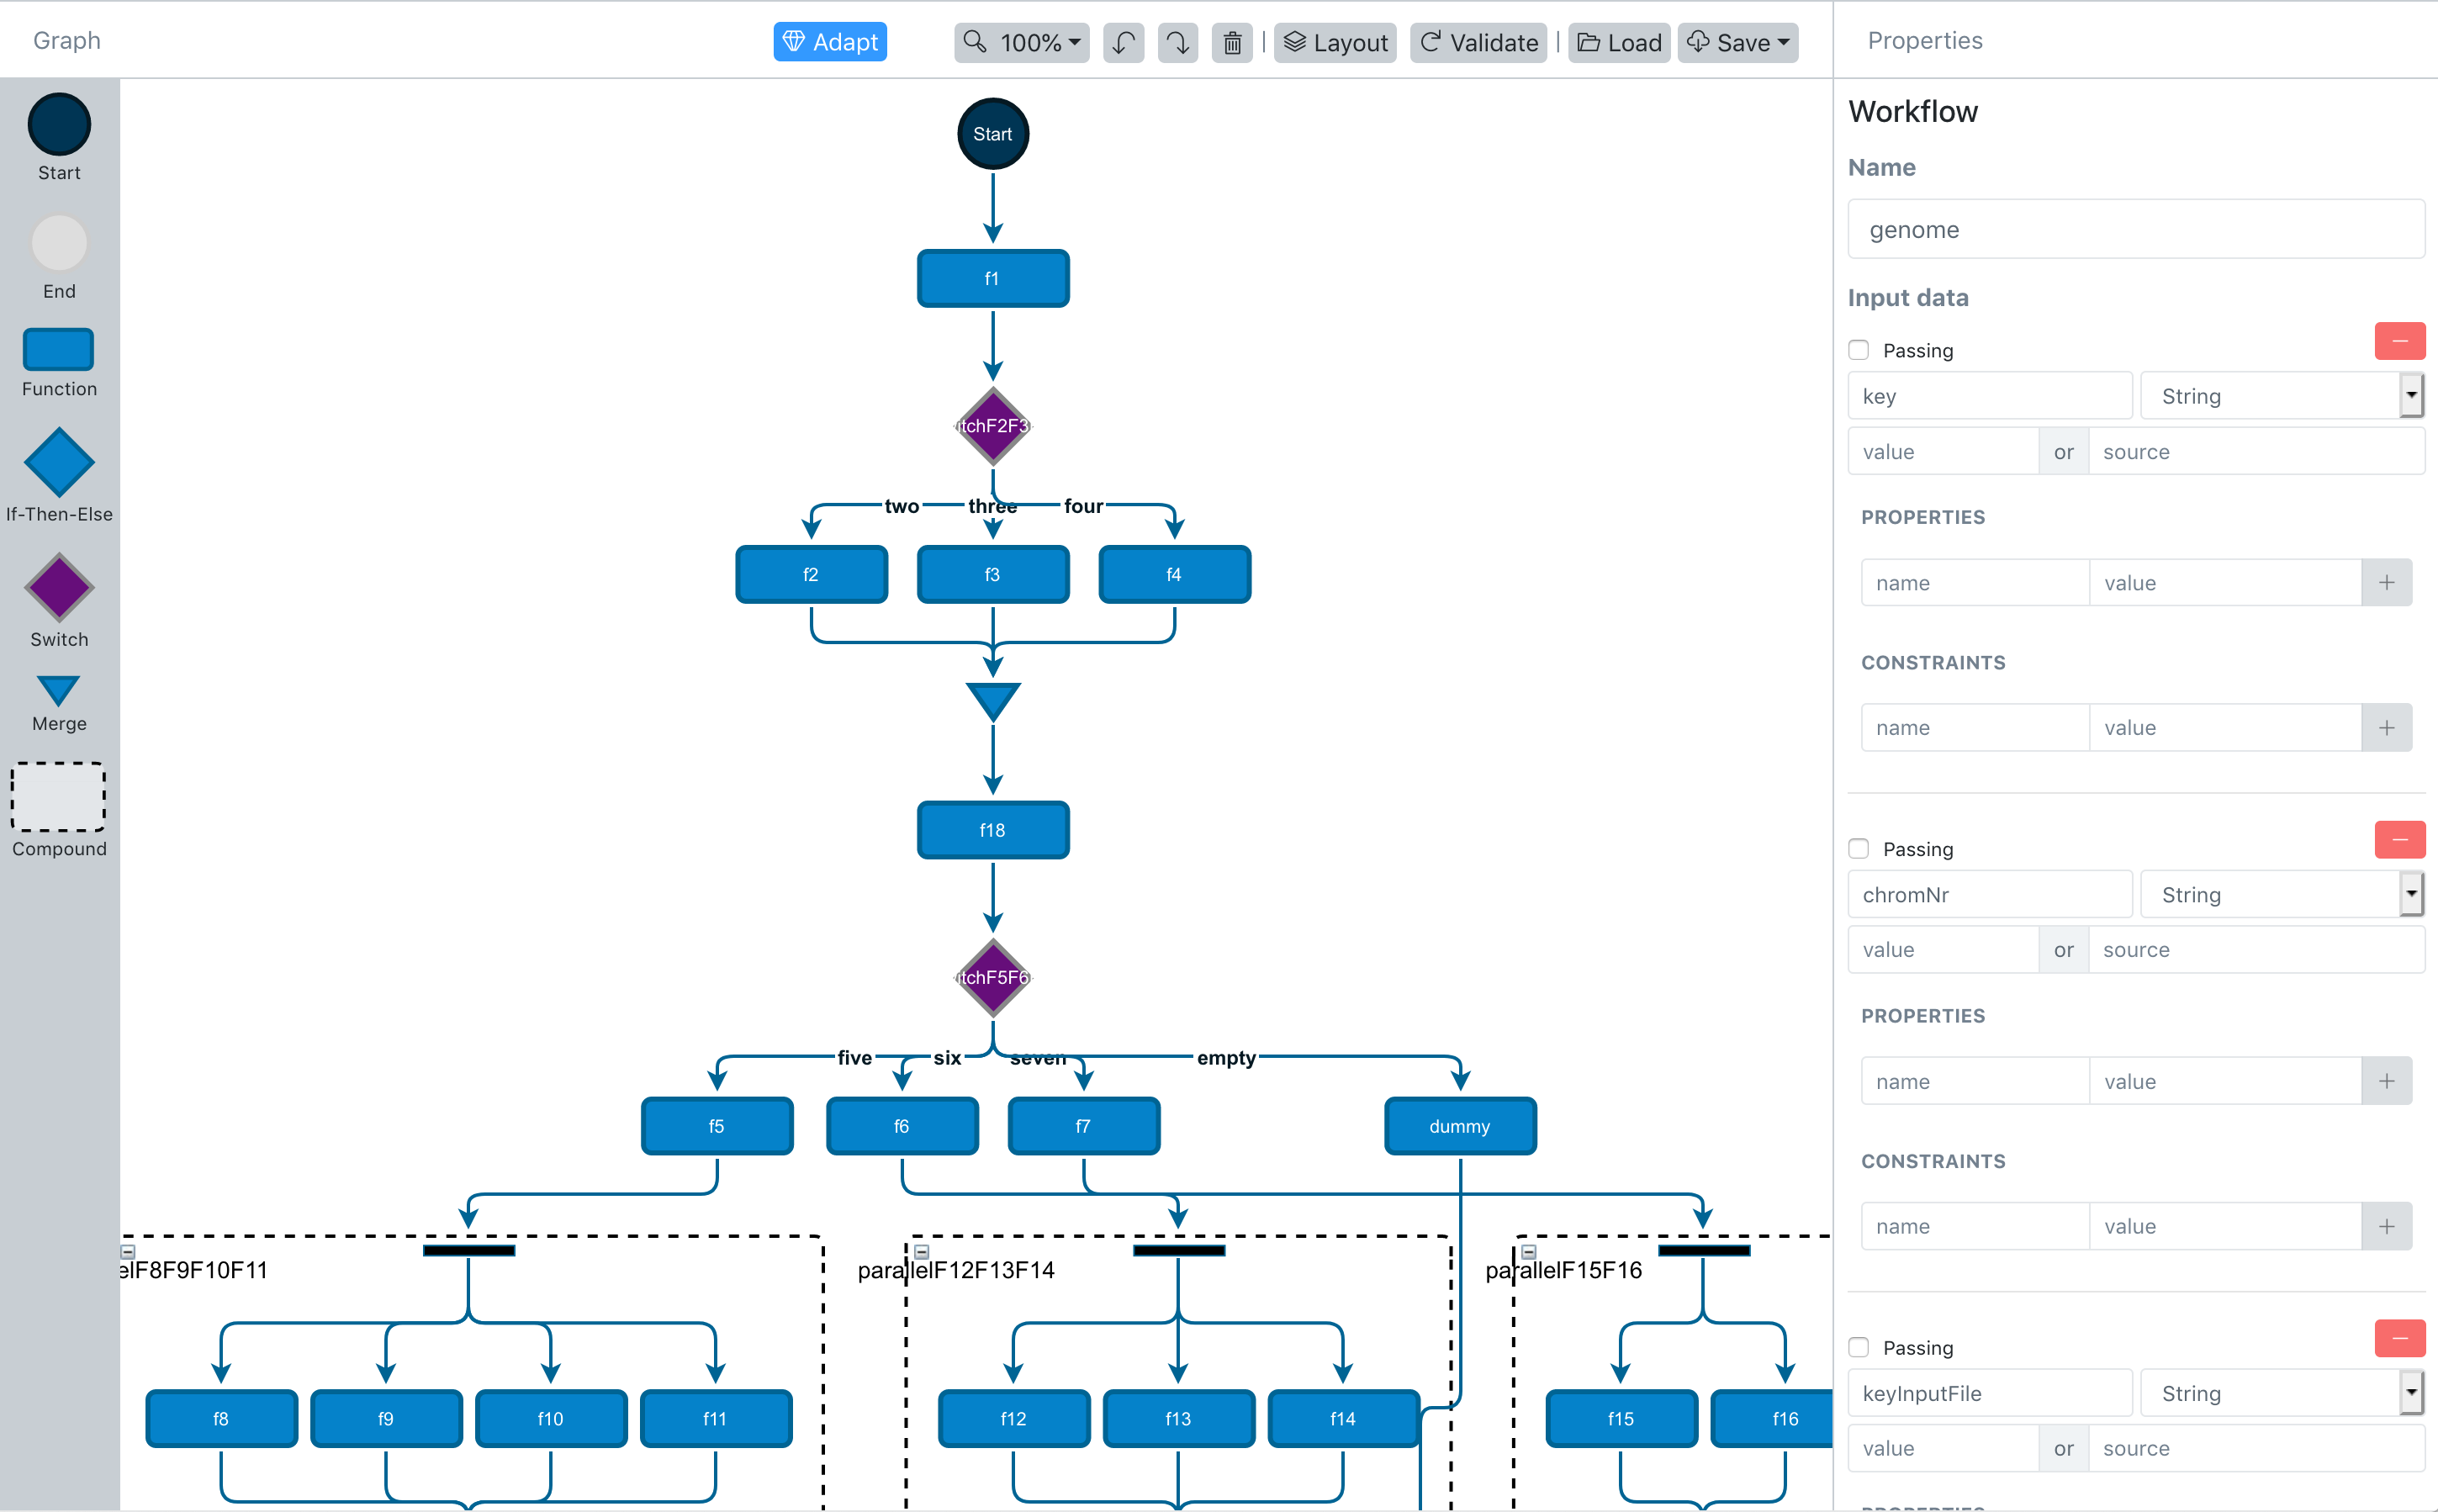
\includegraphics[width=\textwidth]{editor}
  \caption{the editor}
\end{figure}

\subsubsection{Settings}

\section{Backend}
\subsection{Setup}
 Maven, Servlets

\subsection{Api}

RESTful (Functions) and RPC-Style (Workflows)
% https://www.smashingmagazine.com/2016/09/understanding-rest-and-rpc-for-http-apis/

\subsection{Decoding}
\label{sec:backend-decoding}
 XML is good because built-in XPath support in Java.

\subsection{Persistence}
\label{sec:backend-persistence}

Composed workflows are saved to the user's file system by offering a download. The user can then choose the target location.
The storing of function data, on the other hand, is abstracted from the user and persisting of the data is handled internally.
An interface\footnote{https://docs.oracle.com/javase/specs/jls/se7/html/jls-9.html} for the repository was created on the backend side to be capable of supporting any data source. The repository which implements the interface in this thesis, stores the serialized data into a file. This could be easily replaced with any other implementation, for example an implementation which stores the data in a DBMS.

\begin{lstlisting}[language=Java, caption=Repository Interface]
public interface Repository<T> {

    public Collection<T> findAll();

    public T findOne(String id);

    public void add(T obj);

    public void remove(T obj);

    public void remove(String id);

    public void update(T obj);
}
\end{lstlisting}

\subsection{Adaptation}

% interface so that someone can update the yaml file based on 
% decision

\chapter{Evaluation}

% benefit for frontend
% manually vs modeling -> what is the benefit
% compare manually vs modeling (time)
% for a workflow of size X benefit is 30%
% more quality typo-safe
% if there is time: paper, how many errors developers do in average -> bugs will be eliminated

% benefit for backend
% split parallel loops to n loops
% realistic example
% company average uses five clouds (paper/website ?)
% how much time would be needed to update manually
% maybe twenty gates will change for a bigger airport
% run multiple workflows each with big number of passengers
% with system update automatically workflows

\chapter{Conclusion and Future Work}

\printbibliography

\end{document} 
